\documentclass[a4paper]{report}
\usepackage[utf8]{inputenc}
\usepackage[T1]{fontenc}
\usepackage{textcomp}

\usepackage{url}

\usepackage{hyperref}
\hypersetup{
    colorlinks,
    linkcolor={black},
    citecolor={black},
    urlcolor={blue!80!black}
}

\usepackage{graphicx}
\usepackage{wrapfig}
\usepackage{adjustbox}
\usepackage{float}
\usepackage[usenames,dvipsnames]{xcolor}

\usepackage{listings}

\lstset{
    language=Python,
    basicstyle=\ttfamily\footnotesize,
    keywordstyle=\color{blue},
    stringstyle=\color{red},
    commentstyle=\color{gray},
    showstringspaces=false,
    frame=single,
    numbers=left,
    numberstyle=\tiny,
    breaklines=true,
    tabsize=4
}

% \usepackage{cmbright}

\usepackage{amsmath, amsfonts, mathtools, amsthm, amssymb}
\usepackage{mathrsfs}
\usepackage{cancel}

\newcommand\N{\ensuremath{\mathbb{N}}}
\newcommand\R{\ensuremath{\mathbb{R}}}
\newcommand\Z{\ensuremath{\mathbb{Z}}}
\renewcommand\O{\ensuremath{\emptyset}}
\newcommand\Q{\ensuremath{\mathbb{Q}}}
\newcommand\C{\ensuremath{\mathbb{C}}}
\let\implies\Rightarrow
\let\impliedby\Leftarrow
\let\iff\Leftrightarrow
\let\epsilon\varepsilon

% horizontal rule
\newcommand\hr{
    \noindent\rule[0.5ex]{\linewidth}{0.5pt}
}

\usepackage{tikz}
% \usepackage{tikzmark}
\usepackage{pgfplots}
\usepackage{tikz-cd}

\usetikzlibrary{calc, arrows.meta, positioning, angles, quotes, patterns}

% theorems
\usepackage{thmtools}
\usepackage{thm-restate}
\usepackage[framemethod=TikZ]{mdframed}
\mdfsetup{skipabove=1em,skipbelow=0em, innertopmargin=12pt, innerbottommargin=8pt}

\theoremstyle{definition}

\makeatletter

\declaretheoremstyle[
    headfont=\bfseries\sffamily\color{ForestGreen!70!black}, bodyfont=\normalfont,
    mdframed={
        linewidth=2pt,
        rightline=false, topline=false, bottomline=false,
        linecolor=ForestGreen, backgroundcolor=ForestGreen!5,
    }
]{thmgreenbox}

\declaretheoremstyle[
    headfont=\bfseries\sffamily\color{NavyBlue!70!black}, bodyfont=\normalfont,
    mdframed={
        linewidth=2pt,
        rightline=false, topline=false, bottomline=false,
        linecolor=NavyBlue, backgroundcolor=NavyBlue!5,
    }
]{thmbluebox}

\declaretheoremstyle[
    headfont=\bfseries\sffamily\color{NavyBlue!70!black}, bodyfont=\normalfont,
    mdframed={
        linewidth=2pt,
        rightline=false, topline=false, bottomline=false,
        linecolor=NavyBlue
    }
]{thmblueline}

\declaretheoremstyle[
    headfont=\bfseries\sffamily\color{RawSienna!70!black}, bodyfont=\normalfont,
    mdframed={
        linewidth=2pt,
        rightline=false, topline=false, bottomline=false,
        linecolor=RawSienna, backgroundcolor=RawSienna!5,
    }
]{thmredbox}

\declaretheoremstyle[
    headfont=\bfseries\sffamily\color{RawSienna!70!black}, bodyfont=\normalfont,
    numbered=no,
    mdframed={
        linewidth=2pt,
        rightline=false, topline=false, bottomline=false,
        linecolor=RawSienna, backgroundcolor=RawSienna!1,
    },
    qed=\qedsymbol
]{thmproofbox}

\declaretheoremstyle[
    headfont=\bfseries\sffamily\color{NavyBlue!70!black}, bodyfont=\normalfont,
    numbered=no,
    mdframed={
        linewidth=2pt,
        rightline=false, topline=false, bottomline=false,
        linecolor=NavyBlue, backgroundcolor=NavyBlue!1,
    },
]{thmexplanationbox}

\declaretheorem[numberwithin=chapter, style=thmgreenbox, name=Definition]{definition}
\declaretheorem[sibling=definition, style=thmredbox, name=Corollary]{corollary}
\declaretheorem[sibling=definition, style=thmredbox, name=Proposition]{prop}
\declaretheorem[sibling=definition, style=thmredbox, name=Theorem]{theorem}
\declaretheorem[sibling=definition, style=thmredbox, name=Lemma]{lemma}
\declaretheorem[sibling=definition, style=thmbluebox,  name=Example]{eg}
\declaretheorem[sibling=definition, style=thmbluebox,  name=Nonexample]{noneg}
\declaretheorem[sibling=definition, style=thmblueline, name=Remark]{remark}




\declaretheorem[numbered=no, style=thmexplanationbox, name=Proof]{explanation}
\declaretheorem[numbered=no, style=thmproofbox, name=Proof]{preuve}
\declaretheorem[style=thmbluebox,  numbered=no, name=Exercise]{ex}
\declaretheorem[style=thmblueline, numbered=no, name=Note]{note}

% \renewenvironment{proof}[1][\proofname]{\begin{replacementproof}}{\end{replacementproof}}

% \AtEndEnvironment{eg}{\null\hfill$\diamond$}%

\newtheorem*{uovt}{UOVT}
\newtheorem*{notation}{Notation}
\newtheorem*{previouslyseen}{As previously seen}
\newtheorem*{problem}{Problem}
\newtheorem*{observe}{Observe}
\newtheorem*{property}{Property}
\newtheorem*{intuition}{Intuition}


\declaretheoremstyle[
    headfont=\bfseries\sffamily\color{RawSienna!70!black}, bodyfont=\normalfont,
    mdframed={
        linewidth=2pt,
        rightline=false, topline=false, bottomline=false,
        linecolor=RawSienna, backgroundcolor=RawSienna!5,
    }
]{todo}
\declaretheorem[numbered=no, style=todo, name=TODO]{TODO}


\usepackage{etoolbox}

\AtEndEnvironment{vb}{\null\hfill$\diamond$}%
\AtEndEnvironment{intermezzo}{\null\hfill$\diamond$}%




% http://tex.stackexchange.com/questions/22119/how-can-i-change-the-spacing-before-theorems-with-amsthm
% \def\thm@space@setup{%
%   \thm@preskip=\parskip \thm@postskip=0pt
% }

\usepackage{xifthen}

\def\testdateparts#1{\dateparts#1\relax}
\def\dateparts#1 #2 #3 #4 #5\relax{
    \marginpar{\small\textsf{\mbox{#1 #2 #3 #5}}}
}

\def\@lesson{}%
\newcommand{\lesson}[3]{
    \ifthenelse{\isempty{#3}}{%
        \def\@lesson{Lecture #1}%
    }{%
        \def\@lesson{Lecture #1: #3}%
    }%
    \subsection*{\@lesson}
    \testdateparts{#2}
}

% fancy headers
\usepackage{fancyhdr}
\pagestyle{fancy}

% \fancyhead[LE,RO]{Gilles Castel}
\fancyhead[RO,LE]{\@lesson}
\fancyhead[RE,LO]{}
\fancyfoot[LE,RO]{\thepage}
\fancyfoot[C]{\leftmark}
\renewcommand{\headrulewidth}{0pt}

\makeatother

% figure support (https://castel.dev/post/lecture-notes-2)
\usepackage{import}
\usepackage{xifthen}
\pdfminorversion=7
\usepackage{pdfpages}
\usepackage{transparent}
\usepackage[margin=0.8in]{geometry}
\newcommand{\incfig}[1]{%
    \def\svgwidth{\columnwidth}
    \import{./figures/}{#1.pdf_tex}
}

% %http://tex.stackexchange.com/questions/76273/multiple-pdfs-with-page-group-included-in-a-single-page-warning
\pdfsuppresswarningpagegroup=1
\pgfplotsset{compat=1.11}
\usepackage{subcaption}

\author{Yehor Korotenko}

\newcommand{\scalar}[2]{\langle #1, #2 \rangle}
\newcommand{\scalair}[1]{\left\langle #1 \right\rangle}

% fancy chapters
\usepackage{lipsum}
\usepackage[Lenny]{fncychap}
\ChNameUpperCase
\ChNumVar{\fontsize{40}{42}\usefont{OT1}{ptm}{m}{n}\selectfont}
\ChTitleVar{\Large\sc}



\title{Anal avec python}
\begin{document}
\maketitle
\tableofcontents
\chapter{cours 1}
\section{Modèles discrètes}
On diésigne par $N(t)$ la population d'individus à l'instant  $t$.\\
Équation du modèle discret:
 \[
     \underbrace{N(t + \Delta t) - N(t)}_{\text{variation de la population}} = \underbrace{n}_{\text{nombre de naissances}} - \underbrace{m}_{\text{nombre de décès}} + \underbrace{ \underbrace{i}_{\text{immigration}} - \underbrace{e}_{\text{émigration}} }_{\text{sol de migration}}
\] 
\subsection{Modèle de croissance géomètrique}
\begin{itemize}
    \item \underline{hypothèse}:
        \begin{itemize}
            \item solde migration nul: i.e $i - e = 0$
            \item nombre de croissance proportionnel à la taille de la population  $\underbrace{n = \lambda \Delta t N(t)}_{\text{taux de natalité}}$
            \item Idem pour le mobre de décès: $\underline{m = \mu \Delta t N(t)}_{\text{taux de mortalité}}$
        \end{itemize}
    \item \underline{Modèle}: On pose $N_n = N(t_n)$ la taille de la population à l'instant  $t_n$.
         \[
             N_{n+1} - N_{n} = \lambda \Delta t N_n - \mu \delta t N_n
        \] 
        on pose $r = \lambda - \mu$
         \begin{align}
             N_{n+1} = ( 1 + r\Delta t )N_n, \qquad n = 0 
        \end{align}
    \item \underline{Solution}: $N_n = (1 + r \Delta t)^{n}N_0, \quad n \in \N$
    \item \underline{Visualisation}: $\Delta t$ fixé
\begin{figure}[H]
   \centering 
   \begin{subfigure}{0.3\textwidth}
       \centering
       \incfig{natalite-superieure}
       \caption{Natalité supérieure\\ à la mortalité}
       \label{fig:natalite-superieure}
   \end{subfigure}
   \begin{subfigure}{0.3\textwidth}
       \centering
       \incfig{natalite-egale}
       \caption{Natalité égale\\ à la mortalité}
       \label{fig:natalite-egale}
   \end{subfigure}
   \begin{subfigure}{0.3\textwidth}
       \centering
       \incfig{natalite-inferieur}
       \caption{Natalité inférieure\\ à la mortalité}
       \label{fig:natalite-inferieur}
   \end{subfigure}
\end{figure}
\end{itemize}
\begin{property}.
    \begin{itemize}
        \item Lorsque $t \to 0$, la population semble tendre vers une courbe $N(t) = N_0 e^{rt}$, solution de $\begin{cases}
                N'(t) = rN(t)\\
                N(0) = N_0
            \end{cases}$ 
        \item Si $r > 0$, la population croît indéfiniment
        \item Si  $r < 0$, il y a extinction de l'éspèce.
    \end{itemize} 
\end{property}
\underline{Inconvenients:}
\begin{enumerate}
    \item Une croissance infinie n'est pas réaliste
    \item Pour être rigoureux, on devrait écrire $E(rN_n)$ i.e partie entière.
\end{enumerate}

\section{Modèles continues}
\underline{Motivation:} L'observation qui prend $\Delta t$ proche de  $0$ aura beaucoup plus d'information. 
 \begin{remark}
   Le modèle de croissance géomètrique 
   \begin{align*}
       &N(t + \Delta t) - N(t) = \lambda \Delta t N(t) - \mu \Delta t N(t)\\
       \implies&\frac{N(t + \Delta t) - N(t)}{\Delta t} = \lambda N(t) - \mu N(t)
   \end{align*}
   en faisant $\Delta t \to 0$
    \[
        N'(t) = \lambda N(t) - \mu N(t)
    \] 
    D'où l'équation des modèles continues:
    \[
        \underbrace{N'(t)}_{\text{vitesse de variation}} = \underbrace{n(t)}_{\text{vitesse de naissance}} - \underbrace{m(t)}_{\text{vitesse de décès}} + \underbrace{i(t)}_{\text{vitesse d'immigration}} - \underbrace{e(t)}_{\text{vitesse d'émigration}}
    \] 
\end{remark}
\subsection{Modèle de Malthus}
\begin{itemize}
    \item \underline{hypothèse}: 
        \begin{itemize}
            \item solde migration nul: $i(t) - e(t) = 0$
            \item vitesse de naissance proportionnel à la population à l'instant  $t$:  $n(t) = \lambda N(t)$
            \item vitesse de décès: $m(t) = \mu N(t)$
        \end{itemize}
    \item \underline{Modèle}: $\begin{cases}
        N'(t) = (\lambda - \mu)N(t)\\
        N(0) = N_0
    \end{cases}$
\item \underline{Solution}: $N(t) = N_0e^{(\lambda - \mu)t}$
\item 
    \begin{property}
       \begin{itemize}
           \item Il peut être si comme limite du modèle de croissance géomètrique.
           \item Lorsque $r = \lambda - \mu > 0$ croissance est proportionnel.
           \item Lorsque  $r = \lambda - \mu = 0$ la population n'évolue pas.
           \item Lorsque  $r = \lambda - \mu < 0$ la population tend vers 0.
       \end{itemize} 
    \end{property}
\item \underline{Inconvenients}:
    \begin{itemize}
        \item croissance exponentielle pas réaliste. Il faut prendre en compte:
            \begin{itemize}
                \item la limitation des ressources
                \item l'interaction avec l'environnement
            \end{itemize}
    \end{itemize}
\end{itemize}
\subsection{Modèle Verhulst}
Corrige le modèle de Malthus en prennant en compte la limitation de ressources.
\begin{itemize}
    \item \underline{Idée}: limiter la croissance à un seuil $K$ appelé capacité biotique
\begin{figure}[H]
    \centering
    \incfig{malthus-prendre-en-compte}
    \caption{Modèle de Malthus}
    \label{fig:malthus-prendre-en-compte}
\end{figure}
\begin{figure}[H]
    \centering
    \incfig{verhulst}
    \caption{Modèle de Verhulst}
    \label{fig:verhulst}
\end{figure}
\item \underline{hypothèse}: Sole de migration nul
    \begin{itemize}
        \item taux de natalité fonction afiine décroissante de la population $\lambda \approx \lambda (1 - \frac{N(t)}{K})$ 
        \item taux de mortalité fonction affine croissante de la population $\mu \approx -\mu (1 - \frac{N(t)}{K})$
    \end{itemize}
\item \underline{Modèle}: $\begin{cases}
    N'(t) = rN(t)(1 - \frac{N(t)}{K})\\
    N(0) = N_0
\end{cases}$
\item \underline{Solutions}: $N(t) = \frac{K}{1 + (\frac{K}{N_0} - 1) e^{-rt}}$ \quad $t > 0$ 
\item \underline{Visualisation}:
    \begin{figure}[H]
    \centering
    \incfig{verhulst-visualisation}
    \caption{Verhulst solution}
    \label{fig:verhulst-visualisation}
\end{figure}
\item 
    \begin{property}
    Si $r>0$, on a:
    \begin{itemize}
        \item si $N_0 = 0$ $N_0 = K$ on a: $N(t) = N_0 \, \forall t > 0$
        \item si $0 < N_0 < K$, $N$ croissante
        \item si $N_0 > K$, $N$ décroissante 
        \item $N$ possède une limite si  $N_0 > 0$
            \[
            \lim_{t \to \infty} N(t) = K
            \] 
    \end{itemize}
    \end{property}
\end{itemize}
\section{Modèle de croissance logistique}
C'est un modèle discrét
\begin{itemize}
    \item \underline{hypothèse}: i.e $= 0$\\
         $n - m$ est une fonction affine de la population,  i.e $n - m = r \Delta t N(t)( 1 - \frac{N(t)}{K} )$ 
    \item \underline{Modèle}: On suppose $\Delta t = 1$: On pose  $N_n = N(t_n)$
         \[
        \text{On a:} \begin{cases}
            N_{n+1} - N_n = r N_n (1 - \frac{N_n}{K})\\
            N_0 \text{ donné}
        \end{cases}
        \] 
    \item 
        \begin{property} (À vérifier numeriquement) 
            \begin{itemize}
                \item si $r < 2$, la suite converge vers  $K$ 
                \item si  $2 < r < 2.449$, la suite converge vers un cycle
                \item si  $2.449 < r < 2.57$, la suite est encore un cycle mais plus complèxe
                \item si  $r > 2.57$, la suite devient chaotique
            \end{itemize}
        \end{property}
\end{itemize}


\chapter{cours 2}
\section{Notion de champ de vecteurs associée à une EDO}
\subsection{Généralités et définitions}
Les modèles continus de la dynamique de populations sont des \underline{problèmes de Cauchy} pour les EDO.
\begin{align*}
    \text{(EDO)} \begin{cases}
        y'(x) = f(t, y(t)) &\qquad t \in ]0, \pi[ \\
        y(0) = y_0  
    \end{cases}
\end{align*}
Où \begin{align*}
    y: [0, \pi] &\longrightarrow \R \\
    t &\longmapsto y(t) 
.\end{align*}
\begin{align*}
    f: ]0, \pi[ \times \R &\longrightarrow\R\\
    (t, x) &\longmapsto f(t, x) 
.\end{align*}

\begin{itemize}
    \item Si l'on sait résoudre analytiquement l'EDO (i.e donner l'expression de $t \mapsto y(y)$) alors c'est terminé car il suffit d'étudier la fonction $t \mapsto y(t)$
    \item Si l'on ne sait pas détérminer la solution analytique, \underline{on peut}:
        \begin{enumerate}
            \item s'assurer de \textbf{l'éxistence} et \textbf{l'unicité} de la solution et de sa \textbf{stabilité} vis à vis des données du problème.
            \item Puis analyser les propriétés qualitatives de cette solution pour simple analyse de $f(t, x)$
                \begin{center}
                    \textbf{C'est ici qu'intervient les champs de vecteurs.} 
                \end{center}
        \end{enumerate}
\end{itemize}
Illustations.
\begin{enumerate}
    \item Prenons le modèle de Malthus
        \[
        \begin{cases}
            N'(t) = r N(t), \quad t \in ]0, \pi[\\
            N(0) = N_0
        \end{cases}
        \] 
        On sait que $N(t) = N_0 e^{rt}$
    \item Voici ce que fait python pour traiter $N$.
        \begin{figure}[H]
            \centering
            \incfig{voici-ce-que-fait-python}
            \caption{Ce que fait python}
            \label{fig:voici-ce-que-fait-python}
        \end{figure}
    \item Traitons les vecteurs tangents à la courbe $t \mapsto N(t)$ aux points  $t_n$, $n=0$ 
    \item Si l'on connaît les valeurs minimals et maximales de la solutions on peut avoir l'allure de la solution.
        \begin{figure}[H]
            \centering
            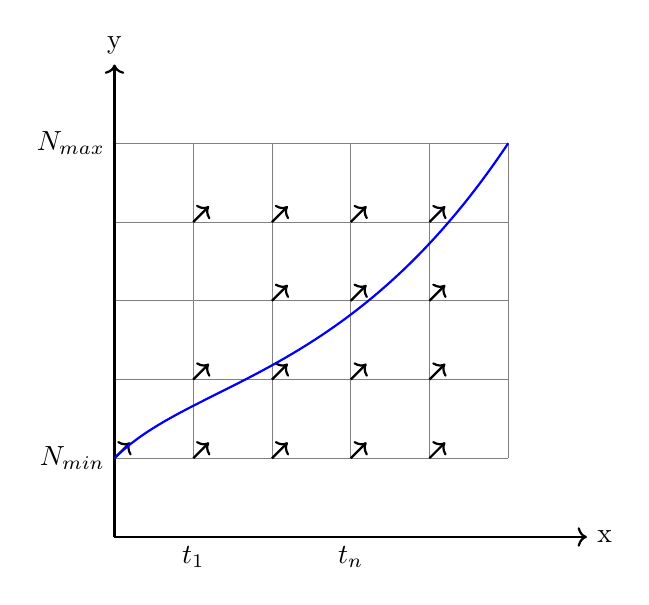
\begin{tikzpicture}
                % Draw the grid
                \draw[step=1cm, gray, very thin] (0,1) grid (5,5);

                % Add axis lines
                \draw[thick,->] (0,0) -- (6,0) node[right] {x};
                \draw[thick,->] (0,0) -- (0,6) node[above] {y};

                \draw[thick,->] (0,1) -- +(0.2, 0.2);
                \draw[thick,->] (1,1) -- +(0.2, 0.2);
                \draw[thick,->] (1,2) -- +(0.2, 0.2);
                \draw[thick,->] (1,4) -- +(0.2, 0.2);
                \draw[thick,->] (2,1) -- +(0.2, 0.2);
                \draw[thick,->] (2,2) -- +(0.2, 0.2);
                \draw[thick,->] (2,3) -- +(0.2, 0.2);
                \draw[thick,->] (2,4) -- +(0.2, 0.2);
                \draw[thick,->] (3,1) -- +(0.2, 0.2);
                \draw[thick,->] (3,2) -- +(0.2, 0.2);
                \draw[thick,->] (3,3) -- +(0.2, 0.2);
                \draw[thick,->] (3,4) -- +(0.2, 0.2);
                \draw[thick,->] (4,1) -- +(0.2, 0.2);
                \draw[thick,->] (4,2) -- +(0.2, 0.2);
                \draw[thick,->] (4,3) -- +(0.2, 0.2);
                \draw[thick,->] (4,4) -- +(0.2, 0.2);
                \node[left] (_) at (0,1){$N_{min}$};
                \node[left] (_) at (0,5){$N_{max}$};
                \draw[thick, blue] (0, 1) .. controls (1,2) and (3,2) .. (5, 5);
                \node[below] (_) at (1, 0){$t_1$};
                \node[below] (_) at (3, 0){$t_n$};
            \end{tikzpicture}  
            \caption{Une courbe sur des champs de vecteurs}
        \end{figure}
\end{enumerate}
Analysons ce que represente le vecteurs tangent:
\begin{itemize}
    \item pour une courbe $y = g(x)$
    \item python et tout autre logiciel procède ainsi
\end{itemize}
\begin{figure}[H]
    \centering
    \incfig{analysons-ce-que-represente-vecteur}
    \caption{Ce que represente vecteur}
    \label{fig:analysons-ce-que-represente-vecteur}
\end{figure}
Le vecteur tangent à la courbe:
\begin{align*}
    \vec{v} = (1, g'(x)) = (1, \frac{dy}{dx}) = (1, \frac{\frac{dy}{dt}}{\frac{dy}{dt}})\\
= \frac{1}{\frac{dy}{dt}}(\frac{dx}{dt}, \frac{dy}{dt}) = \underset{\in \R}{ \frac{1}{\dot{x}(t)} }\underbrace{(\dot{x}(t), \dot{y}(t))}_{\text{vecteur tangent}}
\end{align*}
\[
    \vec{v} = (\dot{x}(t), \dot{y}(t))
\] 
Càd $\vec{v}$ est le vecteur vitesse au points  $M(x(t), y(t))$ a la courbe parametrée  $t \mapsto \begin{cases}
    x(t) = t\\
    y(t) = g(t)
\end{cases}$. On a le résultat.
\begin{prop}
    \begin{align*}
        &\left(\text{y obtient solution de l'EDO } y'(t)=f(t, y(t)) \right) \\
        &\rotatebox{90}{$\iff$}\\ 
        &(\text{vecteur vitesse de la courbe parametrée } t \mapsto (x(t), y(t)) \text{ au point } M(t_0) = (t_0, y(t_0))\\ 
        &\text{ si le vecteur } (1, f(t_0, y(t_0))))  
    \end{align*}
\end{prop}
\begin{prop}
   \begin{align*}
       V: \R^2 &\longrightarrow \R^2 \\
       (t, y) &\longmapsto V((t, y))
   .\end{align*} 
   \[
       \text{(si le champ de vecteur associé à l'EDO } y'(t) = f(t, y(t)) \text{)} \iff V(t, y) = (1, f(t, y))
   \] 
\end{prop}
\subsection{Dessins de champs de vecteurs}
\textbf{\large Principe:}\\
À chaque points $P = (p_x, p_y)$ on trace le vecteur  $\epsilon V(P)$ où  $\epsilon$ est une constance positive choisi pour écrire les vecteurs trop longs.\\
Avec python on écrit \textit{quiver($P_x, P_y, V_x, V_y,$ angles='xy')}
RQ 1: Cette fonction est vectorielle, i.e $P_x, P_y, V_x, V_y,$ sont des numpy array de taille  $n$.
RQ 2: On peut ajouter un paramètre pour controles la longeur des vecteurs:
 \begin{center}
   plt.quiver($P_x, P_y, V_x, V_y$, angles='xy', sacle=$1$) 
\end{center}
Par conséquent, il faut normaliser les vecteurs (i.e le champ de vecteur)
\begin{eg}
   Champ de vecteur du modèle de Verhulst:
   \begin{lstlisting}
       
       def f(t, y):
         return r * y * (1 - y/k)
     \end{lstlisting}
    la grille:

   \begin{lstlisting}
       lt = np.linspace(tmin, tmax, N+1)
       ly = np.linspace(ymin, ymax, M+1)
       T, Y = np.meshgrid(lx, ly)
   \end{lstlisting}
    Construire les vecteurs:

    \begin{lstlisting}
        
       Y = 1 + 0 * T
       V = f(T, Y)
       norm = np.sqrt(U*U + V*V)
        U = U/norm
        V = V/norm
    \end{lstlisting}
    On place les points:
    \begin{lstlisting}
       plt.scatter(T, Y, marker='+', alpha = 0.5)
\end{lstlisting}
    On place les vecteurs
    \begin{lstlisting}
       plt.quiver(T, Y, U, V, angles='xy', scale=N)
\end{lstlisting}
\end{eg}
\subsection{Recherche de solution approchée de modèles sous python}
On cherche une solution approchée de 
\[
\begin{cases}
    y'(t) = f(t, y(t)) \quad t \in ]t_0, t_0 + T[\\
    y(t_0) = y_0
\end{cases}
\] avec python. Pour cela il suffit de dire \textbf{en quels points} on veut cette solution.\\
On se donne:
\begin{itemize}
    \item une liste des instants [$t_0, t_1, \ldots, t_N$]
    \item $t_0, y_0$
    \item Puis, on appelle la fonction \underline{odeint} du module \underline{scipy.integrate} de python.
    \item On obtient une liste [$y_0, y_1, \ldots, y_N$]
\end{itemize}
\begin{eg}
   Cas du modèle du Verhulst 
   \begin{itemize}
       \item EDO:
           \begin{lstlisting}
              def f(t, y):
                return \ldots
           \end{lstlisting}
       \item Instants
           \begin{lstlisting}
              t0, tf = a, b 
              N = 100
              t = np.linspace(t0, tf, N)
           \end{lstlisting}
       \item On appelle odeint
           \begin{lstlisting}
              from scipy.integrate import odeint
              yapp = odeint(f, t, y), rtol=None, atol=None, tfloat=False)
              plt.plot(t, yapp, \ldots)
           \end{lstlisting}
   \end{itemize}
\end{eg}
\section{Modèle de prédateur prose (lotka-voltena (1931))}
$H(t)$: population de sardins\\
$P(t)$: pupulation de reguins
 \[
     \frac{H'(t)}{H(t)} = \text{taux de variation de sardins} = \underbrace{a}_{\text{taux de croissance}} - \underbrace{b P(t)}_{\text{taux de mortalité}}
\] 
\[
    \frac{P'(t)}{P(t)} = \text{taux d'arrivé des requetes} = \underbrace{-c}_{\text{taux de décès}} + \underbrace{d H(t)}_{\text{taux de croissance}}
\] 
D'où le modèle:
\[
\begin{cases}
    H'(t) = H(t)(a - b P(t)) \quad t>0\\
    P'(t) = P(t)(-c + d H(t))\\
    H(0) = H_0, \quad P(0) = P_0
\end{cases}
\] 
Si l'on désigne par $p\ge 0$ la proportion des requêtes en sardines pêchés
\[
\begin{cases}
    H'(t) = H(t)(a - p - b P(t)) \quad t > 0\\
    P'(t) = P(t)(-c - p - d H(t))\\
    H(0) = H_0\\
    P(0) = P_0
\end{cases}
\] 


\chapter{cours3:\\Interpolation polynomiale}
On va essayer de construire des polynôms qui passent par un ensemble (nuages) de points donnés.

Si ces points sont les valeurs d'une fonction, on amerait:
\begin{itemize}
    \item savoir si le polynôme construit est d'autant plus proche de la fonction que le nombre de point est grand. C'est-à-dre, est-ce que nute des "erreurs" tend vers zero lorsque le nombre de points tend vers l'infini.
    \item Si oui, comment quantifier cette convergence? C'est-à-dire, quelle est la vitesse (ordre) de cette convergence.
        \begin{figure}[H]
            \centering
            \incfig{evolution-de-population-en-annee}
            \caption{evolution-de-population-en-annee}
            \label{fig:evolution-de-population-en-annee}
        \end{figure}
\end{itemize}
\begin{enumerate}
    \item Approche 1: approximation linéaire. 
        \begin{itemize}
            \item Polynôme de degré 1
        \end{itemize}
    \item Approche 2: 
        \begin{itemize}
            \item polynôme de degré 1
            \item approximation quadratique
        \end{itemize}
    \item Approche 3: prise en compre d'Historique
\end{enumerate}

\section*{Rappels sur les nuts numériques\\
          Vitesse (ordre) de convergence\\
          valeur ajoutée par itérations
      }
\begin{definition}
    Soit $(x_n)_n \subset \R^n$ une suite qui converge vers $x^* \in \R^n$, pour une norme $\| \, \|$ de  $\R^n$
    \begin{itemize}
        \item Si $k_1 = \lim_{x \to \infty} \frac{\|x_{n+1} - x^*\|}{\|x_n - x^*\|}$ existe et $k_1 \in ]-1, 1[ \setminus \{0\}$. On dit que la suite convere \underline{linéairement} vers $x^*$ ou que la convergence est d'ordre  $1$.
        \item Si  $k_1 = 0$, $k_2 = \lim_{n \to \infty} \frac{\|x_{n+1} - x^*\|}{\|x_n - x^*\|^2}$ existe et non nul. On dit que la suite coverge \underline{quadratiquement} vers $x^*$, ou que la convergence est \underline{d'ordre $2$}.  
        \item Si $k_q = \lim_{n \to \infty} \frac{\|x_{n+1} - x^*\|}{\|x_n - x^*\|^q}$ existe et $\neq 0$ la convergence est \underline{ d'ordre $q$ }. La constante $K_q$ est appelée \underline{constante asymptotique d'erreur}.
    \end{itemize}
\end{definition}
\begin{eg}
    \begin{enumerate}
        \item 
   $x_n = (0.2)^n$ 
   \begin{itemize}
       \item On a $\lim_{n \to \infty} x_n = 0$. La convergence vers $x^* = 0$.
       \item  $\lim_{n \to \infty} \frac{|x_{n+1} - x^*|}{|x_n - x^*|} = \lim_{n \to \infty} \frac{(0.2)^{n+1}}{(0.2)^n} = 0.2 \in ]-1, 1[ \setminus \{0\}$
   \end{itemize}
   D'où
   \begin{itemize}
       \item $x_n$ converge à \underline{l'ordre $1$} 
       \item Sa constante asymptotique est \underline{$k_1 = 0.2$}
   \end{itemize}
   \item
       $I_n = (0.2)^{2^n}$. On a  $\lim_{n \to \infty} I_n = 0$\\
       On a:
       \begin{align*}
           I_{n+1} = (0.2)^{2^{n+1}} &= (0.2)^{2^n \cdot 2}\\
                                     &= \left( (0.2)^{2^n} \right)^2\\
                                     &= \left( I_n \right)^2
       \end{align*}
       D'où $\lim_{n \to \infty} \frac{I_{n+1}}{\left( I_n \right)^2} = \lim_{n \to \infty} \frac{\left( I_n \right)^2}{\left( I_n \right)^2} = 1$
       D'où
       \begin{itemize}
           \item convergence \underline{d'ordre $2$}
           \item de constante $k_2 = 1$
       \end{itemize}
\end{enumerate}
\end{eg}
En pratique, on ne dispose pas de $K_q$
 \begin{definition}
    \[
        \substack{x_n \text{ converge vers } x^*\\\text{à l'ordre } q} \implies \exists N \in \N, \exists A,B \in \R \text{ tq } \forall n \ge N, 0 < A \le \frac{\|x_{n+1} - x^*\|}{\|x_n - x^*\|^q} \le B < +\infty
    \] 
    La convergence est au moins d'ordre $q$ si et seulement si on a (deuxieme partie d'équation)
\end{definition}

\subsection{Valeur ajoutée par l'itération}
Il est question de comparer $2$ suites qui ont la même vitesse de convergence.
\begin{remark}
    Si $|x_n - x^*| = 4 \cdot 10^{-8} = 0.\underbrace{0000000}_{7 \text{ chiffres}}4$. On dira que $x_n$ et  $x^*$ ont 7 chiffres exactes apres la virgule.
    \begin{align*}
    &\log_{10} |x_n - x^*| = \log_{10}4 - 8\log_{10}(10)\\
    &\frac{\log|x_n - x^*}{\log 10} = \frac{\log 4}{\log 10} - 8
    \end{align*}
    i.e $d_n = - \log_{10} |x_n - x^*|$ mesure de nombre de chiffres décimales entre $x_n$ et  $x^*$ qui coincident.
\end{remark}
\begin{remark}
   \[
       \lim_{n \to \infty} \frac{\|x_{n+1} - x^*\|}{\|x_n - x^*\|^q} = K_q \implies K_q \approx \frac{\|x_{n+1} - x^*\|}{\|x_n - x^*\|^q}
   \]  
   D'où $d_{n+1} - q d_n \approx -\log_{10} K_q$, i.e
   \[
   d_{n+1} + \frac{\log_{10} K_q}{1 - q} \approx q(d_n + \frac{\log_{10} K_q}{1 - q})
   \] 
   Donc, le nombre de chiffres significatives est multiplié par $q$.
\end{remark}
\begin{prop}
   Si $x_n$ converge à l'ordre  $1$ vers  $x^*$ de constante asymptotique  $K_1$, alors le nombre d'itérations nécessaires pour gagner un chiffre exacte est la partié enitère de  $-\frac{1}{\log_{10}K_1}$ 
\end{prop}
\begin{preuve}
Soit $m$ le nombre d'itérations pour gegner un chiffre. Comme  $d_{n+1} - d_n = -\log_{10} K_1$, en partant de $d_n$, après  $m$ itérations on aura
 \[
     d_{n+m} - d_{n} = -m \log_{10}K_1
\] 
D'où on aura gagné $1$ chiffre si  $d_{n+m} - d_n = 1$, i.e
\[
1 = -m \log_{10}K_1 \implies m = \left( -\frac{1}{\log_{10}K_1} \right) 
\] 
\end{preuve}

\subsection{Obtenir numériquement la vitesse de convergence}
On cherche $q$ tq:  $\lim_{n \to \infty} \frac{\|x_{n+1} - x^*\|}{\|x_n - x^*\|^q} = K_q \in  \R^*$
\begin{remark}
    \begin{align*}
        &\frac{\|x_{n+1} - x^*\|}{\|x_n - x^*\|^q} \approx K_q
        \implies& \underbrace{ \log \|x_{n+1} - x^*\|  }_{Y} - \underbrace{q \log\|x_n - x^*\|}_{X} = \log K_q
    \end{align*}
    i.e $Y = aX + b$. 
    \par
    Conclusion: pour détérminer q:
     \begin{itemize}
        \item Traiter la courbe $\log\|x_n - x^*\| \mapsto \log\|x_{n+1} - x^*\|$
        \item Détérminer $q$ comme la parte de la droite passant par le maximum de points.
    \end{itemize}
\end{remark}
\begin{align*}
    &x_n = x_0, x_1, \ldots, x_N\\
    &x_n - x^* = x_0 - x^*, x_1 - x^*, \ldots, x_N - x^*\\
    &x_{n+1} - x^* = x_1 - x^*, x_2 - x^*, \ldots, x_{N+1} - x^*
\end{align*}
En python:

\begin{lstlisting}
xn = np.array([x0, ..., xN])
e = np.log(np.abs(xn - x^*))
ex = e[0:-1] #de premier a avant dernier
ey = e[1:] #de deuxieme au dernier
plt.scatter(ex, ey, label="miage")
a,b = np.polyfit(ex, ey, 1)
plt.plot(ex, b + a * ex, label=f"$x \mapsto {b:32f} + {a:32f}x$")
\end{lstlisting}
\end{document}

